
\documentclass[12pt]{article}
\pagestyle{empty}
\setlength{\parskip}{0in}
\setlength{\textwidth}{6.8in}
\setlength{\topmargin}{-.5in}
\setlength{\textheight}{9.3in}
\setlength{\parindent}{0in}
\setlength{\oddsidemargin}{-.7cm}
\setlength{\evensidemargin}{-.7cm}

\usepackage{amsmath}
\usepackage{amsthm}
\usepackage{amstext}

\usepackage{graphicx}

\begin{document}

{\bf MAT 105 Final Exam (ivory) Fall 2009} \hspace{.4in} {\large Name} \hrulefill

\hspace{.2in}

\begin{center}

\begin{tabular}
{|l|c|c|c|c|c|c|c|c|c|c|c|c|c|c|c|c|} \hline

 Problems & \hspace{5 pt} 1 \hspace{5 pt}  & \hspace{5 pt} 2 \hspace{5 pt} & \hspace{5 pt} 3 \hspace{5 pt} & \hspace{5 pt} 4 \hspace{5 pt}& \hspace{5 pt} 5 \hspace{5 pt} & \hspace{5 pt} 6 \hspace{5 pt} & \hspace{5 pt} 7 \hspace{5 pt}   & \hspace{5 pt} 8 \hspace{5 pt} &  \hspace{5 pt} Total  \hspace{5 pt} & &  \hspace{5 pt} Grade \hspace{5 pt}  \\ \hline
&&&&&&&&&&&\\  
Points &&&&&&&&&&   \hspace{.6in}\% &  \\ 
&&&&&&&&&&& \\  \hline
Out of & 40  & 14 & 28 & 22 & 38 & 17 & 22 & 19 &200 & & \\ \hline

\end {tabular}
 
\end{center}

\hspace{.2in}

\begin{itemize}
\item Relax.  You have done problems like these before. Even if these problems look a bit different, just do what you can. 
\item  If you're not sure of something or if you're stuck, please ask! 
\item You may use your calculator but please show all of your work and write down as many steps as you can.  
\item Some formulas from our book that you might need are on a separate sheet.
\item Don't spend too much time on any one problem.
\item  Do well.  And remember to ask me if you need help.
\end{itemize}

  \vspace{.2in}
 
 \hrulefill
 
\newpage  %%%

\begin{enumerate}
\item Evaluate each of the following expressions.

\begin{enumerate}
\item $49.99 + 1.07(300)=$
\vfill
\item $(20)^2-4(-5)(3)=$
\vfill
\item $2,400(1.06)^{72}=$
\vfill
\item $\displaystyle \frac{-(20)}{2(-5)}=$
\vfill
\item $2^{30}=$
\vfill
\item $(9.2)^{1/4}=$
\vfill
\item $\sqrt{179}=$
\vfill
\item $\displaystyle \frac{\text{log}(29.22)}{\text{log}(1.04)}=$
\vfill
\emph{Write the next answer in normal (expanded) decimal notation.}
\item $5.38 \times 10^{17}=$  


\vfill
\emph{Write the next answer in normal (expanded) decimal notation.}
\item $5.38 \times 10^{-17}=$  


\vfill
\end{enumerate}

\newpage  %%%

\item The 1918 flu season was one of the deadliest in history.  The graph and table show the number of flu deaths in England during 1918.

\begin{center}
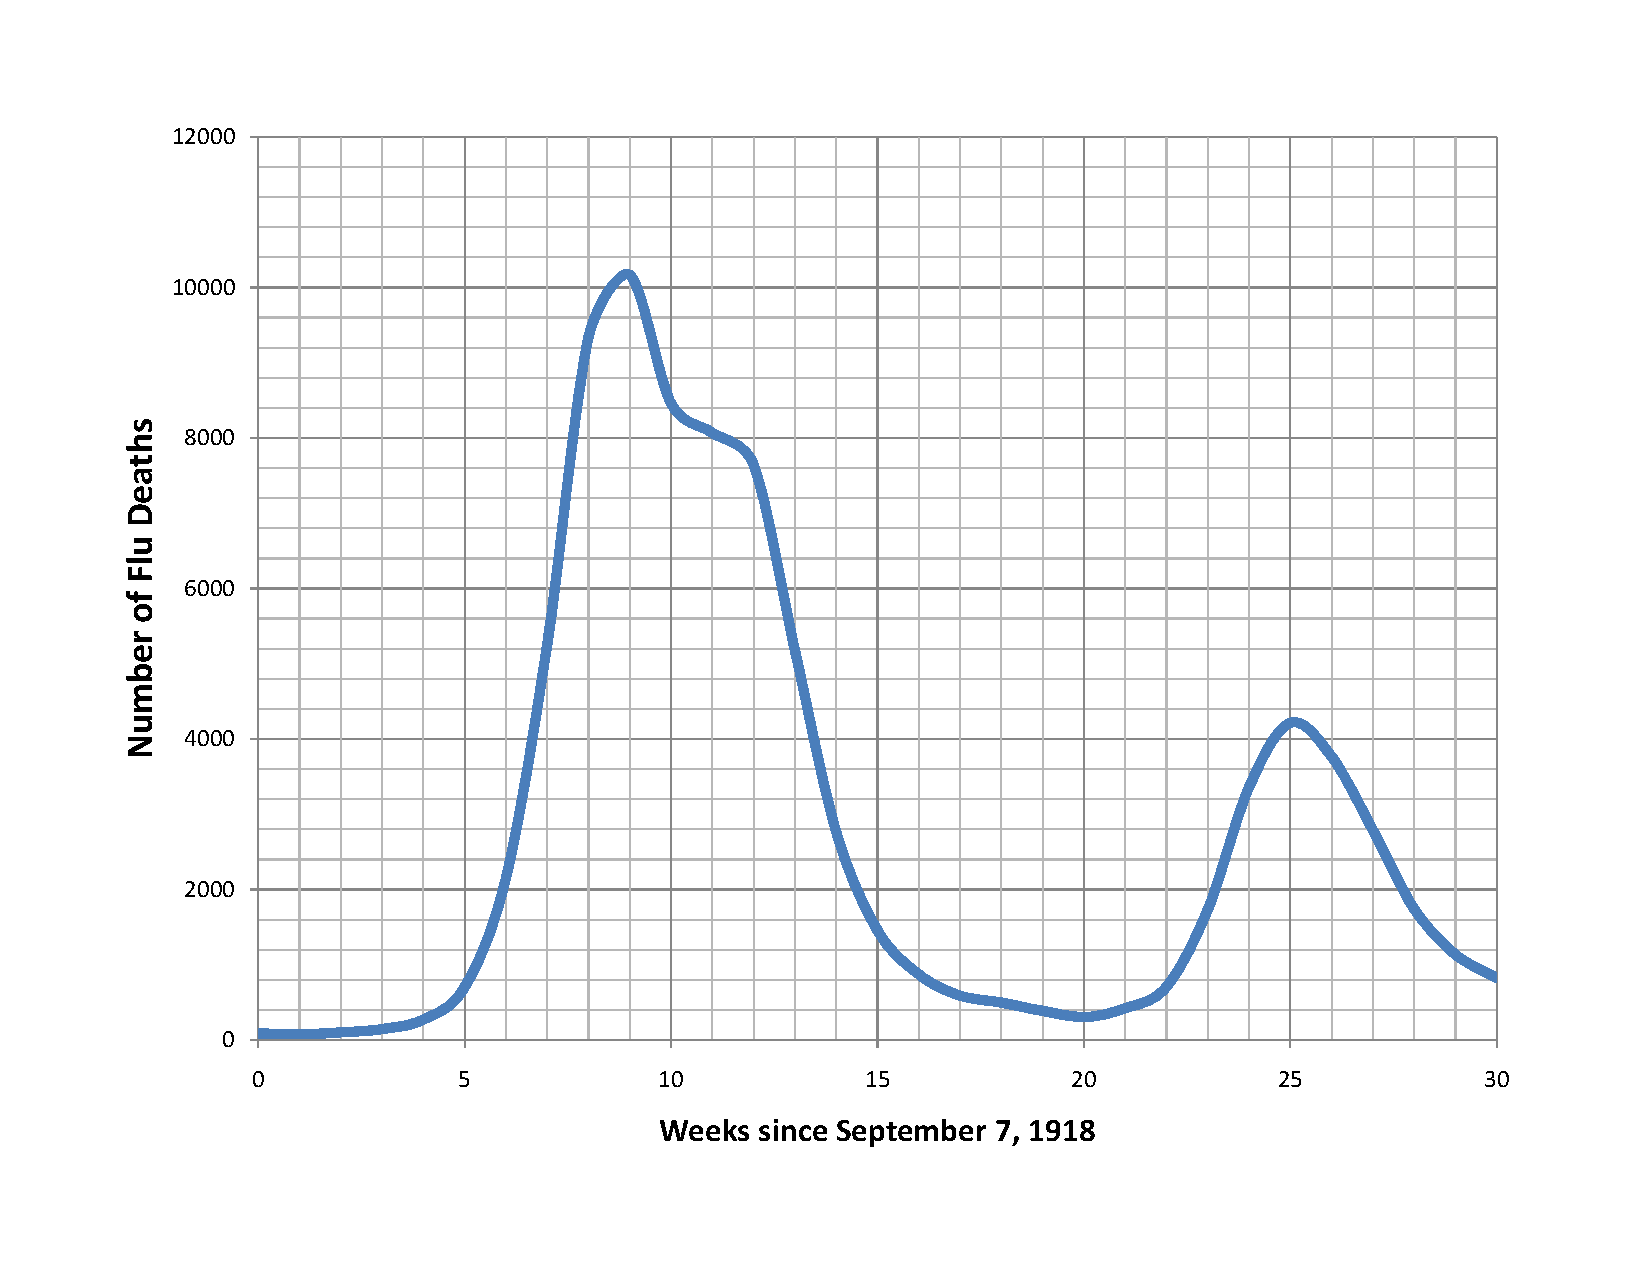
\includegraphics [width = .7\textwidth] {EnglandFlu.pdf}
\end{center}

\begin{tabular} {|c|c|c|c|c |c|c|c|c|c |c|c|} \hline
Weeks since Sept. 7, 1918 & 0 & 3 & 6  & 9  & 12  & 15  & 18 & 21  & 24  & 27  & 30 \\ \hline
Number of deaths &90 & 145 & 2148 & 10168 & 7642 & 1460 & 498 & 423 & 3360 & 2791 & 822 \\ \hline
\end{tabular}

\begin{enumerate}
\item How many people died from the flu 6 weeks after September 7?
\vfill
\item In what week after September 7 did the number of flu deaths drop back to the level at 6 weeks?
\vfill
\item In what week after September 7 was the number of flu deaths the highest and what were the approximate number of deaths?
\vfill
\item Was the number of weekly flu deaths increasing faster 6 weeks after September 7 or 24 weeks after September 7?  Explain. (\emph{Hint: Determine the average rate of change at both of these times.})
\vfill
\end{enumerate}

\newpage %%%

\item My mechanic charges $M$ dollars for $H$ hours of work, as given by the following formula:
$$M = 29.95 + 50.00H$$

\begin{enumerate}
\item Make a table of values showing the charges for 1 hour, 1$\frac{1}{2}$ hours, 2 hours, and 3 hours.
\vfill
\item What does the 29.95 represent and what are its units?
\vfill
\item What does the 50.00 represent and what are its units?
\vfill
\item If the bill for my last visit to the mechanic was $\$317.45$, how much time did he work?

\emph{Set up and solve an equation to answer the question.  If you can't solve it, then you may estimate the answer to two decimal places for possible partial credit.}
\vfill
\vfill
\vfill
\item Convert your answer to the nearest minute.
\vfill
She worked for \hrulefill hours, \hrulefill minutes. \hspace{3in}.
\end{enumerate}

\newpage %%%
%% http://aa.usno.navy.mil/data/docs/RS_OneYear.php
\item The timing of the sunset depends on the latitude (how far North of South of the equator one is) and the time of year.  In Minneapolis, the sunset occurred at 4:43 PM on January 1.  The time of the sunset is expected to occur 1.19 minutes later each day.  In Panama City, Florida, the sunset occurred at 4:54 PM on January 1 and is expected to occur 0.81 minutes later each day.  (Note: do not worry about Daylight Savings Time.) If we let $S$ represent the time of the sunset (in minutes after 4 PM) for $D$ days since January 1, then the equations are:

\vspace{.1in}

\begin{center}
\begin{tabular} {ll} 
Minneapolis: &$S=43+1.19D$ \\
Panama City: & $S=54+0.81D$ \\
\end{tabular}
\end{center}

The table shows sunset times for the two cities:

\begin{center}
\begin{tabular} {|l|r|r|r|r|} \hline
$D$ & 0 & 5 & 15 & 31 \\ \hline
$S$ (Minneapolis) & 43 &  49.0 & 60.9 & 79.9  \\ \hline
$S$ (Panama City) & 54 & 58.1 & 66.2 & 79.1 \\ \hline
\end{tabular}
\end{center}

\begin{enumerate}

\item Which city has a later sunset on January 10 (i.e. after 10 days)?  \emph{Justify your answer.}
\vfill

\item Draw a graph illustrating both equations.
\vspace{.1in}
\begin{center}
\scalebox {.8} {
\includegraphics [width = 6in] {../GraphPaper}}
\end{center}
\vfill
\emph{The problem continues on the next page ...}
\pagebreak
\item Set up and solve an equation to find when the two cities will have the sunset at the same time. Report your answer to the nearest day.

\emph{Just approximating the answer will get almost no partial credit.}

\vfill
\vfill
\vfill
\end{enumerate}

\newpage %%%

\item Peter jumped from a rock into an abandoned mining pit filled with water. The rock ledge was 4 meters above the ground.  His height above the water, $H$ meters, after $T$ seconds is given by the formula: $$H = 4 + 6.2T - 4.88T^2$$

\begin{enumerate}
\item Complete the following table of values.

\emph{Please report your answers to the first two decimal places.}

\begin{center}
\begin{tabular} {|l|c|c|c|c|c|c|} \hline
$T$ & 0 & 0.3 & 0.5 & 0.8 & 1.0 & 1.4 \\ \hline
&&&&&& \\
$H$ & \hspace{.7in} & \hspace{.7in}  & \hspace{.7in}  & \hspace{.7in}  & \hspace{.7in}  & \hspace{.7in}  \\
&&&&&& \\ \hline
\end{tabular}
\end{center}

\item How high up in the air does Peter get?

\emph{Find the answer to two decimal places using whatever method you prefer.}
\vfill
\vfill

\item Convert your answer to the nearest foot.  \emph{Use 1 meter = 3.28 feet.}
\vfill

\hspace{-.5in} \emph{The problem continues on the next page.}

\newpage %%%

\item Draw a graph illustrating the dependence.

\vspace{.1in}
\begin{center}
\scalebox {.8} {
\includegraphics [width = 6in] {../GraphPaper}}
\end{center}
\vspace{.1in}

\item When does Peter hit the water?

\emph{Find the answer to two decimal places using whatever method you prefer.}

\vfill
\end{enumerate}

\newpage %%%
%%% http://www.energywatchgroup.org/fileadmin/global/pdf/2009-01_Wind_Power_Report.pdf

\item Recent reports indicated that the use of windpower to generate energy is growing exponentially.  In 2006, windpower generated 74,000 Mega-Watts of energy.  A conservative estimate on the growth of windpower is 15.2\% per year.  That is, the energy $E$ (in Mega-Watts) produced by windpower $Y$ years after 2006 is given by the equation:

$$E=74000(1.152)^Y$$

\begin{enumerate}
\item According to this equation, how much energy will be produced from windpower in 2009?
\vfill
\item If the value continues to increase, in what year will windpower generate over 150,000 Mega-Watts of Energy?

\emph{Set up and solve an equation to answer the question.  If you can't solve it, then you may estimate the answer for possible partial credit.}
\vfill
\vfill
\vfill
\end{enumerate}

\newpage %%%

\item I had to rent a tile saw from Home Depot to finish a remodeling project.    The table below lists the rental charges for the saw.  They charge an initial fee plus an hourly rate.

\begin{center}
\begin{tabular} {|r|r|r|r|r|r|r|} \hline
Hours & 1 & 2 & 3 & 4 & 5 & 10 \\ \hline
Cost & \$35.90 & \$51.85 & \$67.80 & \$83.75 & \$99.70 & \$179.45 \\ \hline
\end{tabular}
\end{center}

\begin{enumerate}
\item Name the variables including units.
\vfill
\item What does the Home Depot charge per hour for the tool rental?
\vfill
\item What is the initial fee?
\vfill
\item Write an equation describing the cost of renting a tile saw.
\vfill
\end{enumerate}

\newpage %%%
%%% http://en.wikipedia.org/wiki/List_of_newspapers_in_the_United_States_by_circulation
%%% http://www.infoplease.com/ipea/A0004420.html
\item Newspaper subscriptions have dropped as more people use the internet for news.  In 2006, the Minneapolis Star Tribune had 606,698 subscribers.  Today in 2009 (3 years later), only 322,360 people subscribe to the paper. You can assume that the decline is exponential.

\begin{enumerate}
\item By what percentage has the number of subscribers dropped each year?
\vfill
\item If this trend continues, what will the number of subscribers be in 2012 (i.e.\ after 6 years from 2006)?
\vfill
\end{enumerate}



\end{enumerate}

\end{document}

